{}

\section{{Problem 1}}

	{The error form to the 13 faulty buggy programs are as follows.}

	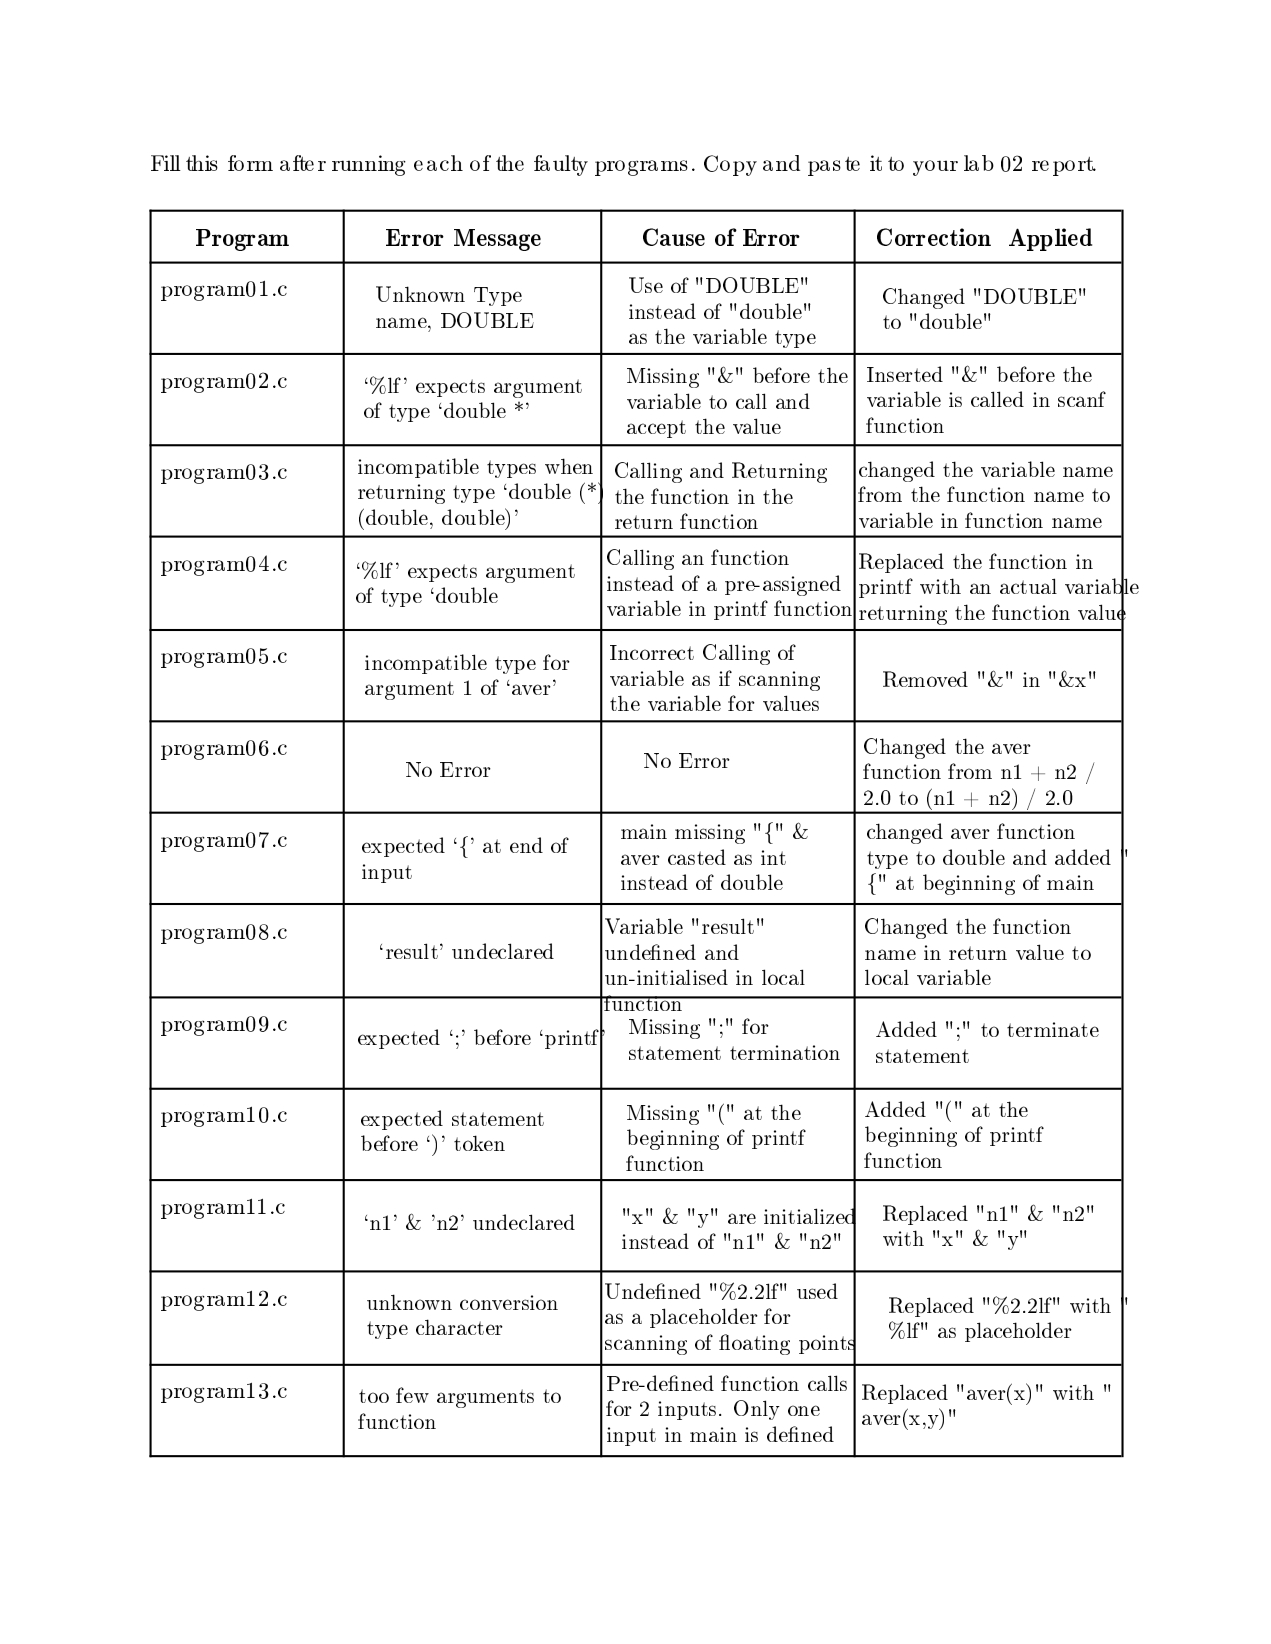
\includegraphics[width=12.75cm]{Error Form.jpg}

	{}

%\clearpage

%\section{{Problem 2}}

%	\subsection{{Computer Program}}

%		\begin{lstlisting}[language=C, caption=\textit{Hello World Program}]	
%/* My first C program */

%#include <stdio.h>

%int main (void)
%{
%   printf ("This is my first C program.\n");
%   return (0);
%}


%\end{lstlisting}

%	\subsection{{Program Output Screenshot}}

%		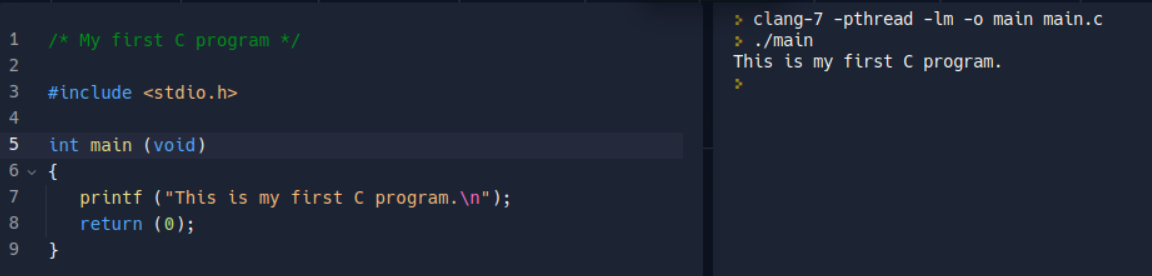
\includegraphics[width=15cm]{Hello World.png}
		
\section{{Problem 2}}

		\subsection{{Algorithm}}	
	
		\begin{itemize}
			\item {Declare, Scan and store value temperature in Celsius}
			\item {Convert Celsius temperature to Fahrenheit temperature}
			\item {Substutitute the Fahrenheit temperature in the formula}
			\item {convert the formula speed from ft/s to km/h}
			\item {Print the km/h speed as output to user}
			%\item {Multiply the two scaned values and divide by two. Return the following vaule of the operation as the area.}
		\end{itemize}
	
		\subsection{{Computer Program}}
	
			\begin{lstlisting}[language=C, caption=\textit{Speed of Sound Calculating Program}]	
/*  Program to Calculate the speed of sound given some Temperature Input    */

#include <stdio.h>
#include <math.h>

void spsound(void);

int main(void)
{
    spsound();
}

void spsound(void)
{
    /*  Celcius temperature input   */
    double celsius;
    printf("Enter the Temperature of Air: ");
    scanf("%lf", &celsius);

    /*  Celsius to Fahrenheit Conversion    */
    double fahrenheit = ((celsius * 9) / 5) + 32;

    /*  Speed of Air calculation    */
    double speed = 1086 * sqrt((5 * fahrenheit + 297) / 247);

    /*  ft/s to km/h Conversion of speed    */
    speed = speed * 1.09728;

    /*  Printing the speed as the function output*/
    printf("\nThe Speed of the Air at %.3lf Celsius is %.3lf km/h\n", celsius, speed);
}




		\end{lstlisting}
